% Images
\pgfdeclareimage[width=10cm]{ROSEquation}{./images/ros_equation_2}
\pgfdeclareimage[width=10cm]{gazebo}{./images/gazebo_horz_cmyk_pos.jpg}
\pgfdeclareimage[width=10cm]{opencv}{./images/opencv_logo.png}
\pgfdeclareimage[width=10cm]{pcl}{./images/pointcloudlibrary_horz_large_pos.jpg}
\pgfdeclareimage[width=10cm]{moveit}{./images/moveit-logo.png}

\pgfdeclareimage[width=2cm]{ros-ubuntu-logo}{./images/ros-ubuntu-logo.png}

\pgfdeclareimage[width=2cm]{ros-ubuntu-arm-logo}{./images/ros-ubuntu-arm-logo.png}
\pgfdeclareimage[width=2cm]{ros-os-x-homebrew-logo}{./images/ros-os-x-homebrew-logo.png}
\pgfdeclareimage[width=2cm]{ros-os-x-macports-logo}{./images/ros-os-x-macports-logo.png}

\pgfdeclareimage[width=2cm]{ros-yocto-logo}{./images/ros-yocto-logo.png}
\pgfdeclareimage[width=2cm]{ros-debian-logo}{./images/ros-debian-logo.png}
\pgfdeclareimage[width=2cm]{ros-arch-linux-logo}{./images/ros-arch-linux-logo.png}

\pgfdeclareimage[width=2cm]{ros-windows-logo}{./images/ros-windows-logo.png}
\pgfdeclareimage[width=2cm]{ros-angstrom-logo}{./images/ros-angstrom-logo.png}
\pgfdeclareimage[width=2cm]{ros-udoo-logo}{./images/ros-udoo-logo.png}

\pgfdeclareimage[width=2cm]{ros-arch-linux-logo}{./images/ros-arch-linux-logo.png}

\pgfdeclareimage[width=2cm]{ros-nao}{./images/nao.jpg}
\pgfdeclareimage[width=3cm]{ros-turtlebot}{./images/robot-turtlebot2-front.jpg}
\pgfdeclareimage[width=3cm]{ros-motoman}{./images/motomanSIA10D.jpg}

\pgfdeclareimage[width=4cm]{rviz}{./images/rviz.png}
\pgfdeclareimage[width=4cm]{rosbag-slam}{./images/rosbag-slam.png}
\pgfdeclareimage[width=4cm]{rxplot}{./images/rxplot.png}
\pgfdeclareimage[width=4cm]{rxgraph}{./images/rxgraph_turtle_key.png}
\pgfdeclareimage[width=4cm]{rqt}{./images/rqt.jpg}


% Tikz libraries
\usetikzlibrary{shadows}
\usetikzlibrary{automata}
\usetikzlibrary{arrows}
\usetikzlibrary{trees}
\usetikzlibrary{positioning}

% For arrows
\definecolor{darkblue}{rgb}{0.2,0.2,0.6}
\definecolor{darkred}{rgb}{0.6,0.1,0.1}
\definecolor{darkgreen}{rgb}{0.2,0.6,0.2}

\def\arrowt{
  (0.1,0.5) -- (0.0,1) -- (6.0,1.0) [rounded corners=0.5] --
  (6.0,1.5) [rounded corners=1] -- (7.0,0.5) [rounded corners=0.5] --
  (6.0,-0.5) [sharp corners] -- (6.0,0.0) -- (0.0,0.0)
  [rounded corners=1] -- (0.1,0.5) -- cycle
}

\def\arrowd{
  (10.75:1.1) -- (6.5:1) arc (6.25:120:1) [rounded corners=0.5] --
  (120:0.9) [rounded corners=1] -- (130:1.1) [rounded corners=0.5] --
  (120:1.3) [sharp corners] -- (120:1.2) arc (120:5.25:1.2)
  [rounded corners=1] -- (10.75:1.1) -- (6.5:1) -- cycle
}

\def\arrow{
  (10.75:1.1) -- (6.5:1) arc (6.25:90:1) [rounded corners=0.5] --
  (90:0.9) [rounded corners=1] -- (100:1.1) [rounded corners=0.5] --
  (90:1.3) [sharp corners] -- (90:1.2) arc (90:5.25:1.2)
  [rounded corners=1] -- (10.75:1.1) -- (6.5:1) -- cycle
}

\def\arrowtd{
  (-10.75:1.1) -- (-6.5:1) arc (-6.25:-170:1) [rounded corners=0.5] --
  (-170:0.9) [rounded corners=1] -- (-180:1.1) [rounded corners=0.5] --
  (-170:1.3) [sharp corners] -- (-170:1.2) arc (-170:-5.25:1.2)
  [rounded corners=1] -- (-10.75:1.1) -- (-6.5:1) -- cycle
}

\tikzset{
  ashadow/.style={opacity=.25, shadow xshift=0.07, shadow yshift=-0.07},
}


\def\arrows[#1]{         
  \begin{scope}[scale=#1]
    \draw[color=darkred, %
    drop shadow={ashadow, color=red!60!black}] \arrow;

    %\draw[color=darkgreen, bottom color=green!90!black, top color=green!60, %
    %drop shadow={ashadow, color=green!60!black}] [rotate=120] \arrow;

    %\draw[color=darkblue, right color=blue, left color=blue!60, %
    %drop shadow={ashadow, color=blue!60!black}] [rotate=240] \arrow;

    % to hide the green shadow

  \end{scope}
}

\def\motivationpicture{
  \begin{tikzpicture}[remember picture, overlay]
    %HRP-2
    \node[inner sep=0pt,scale=0.5] (hrp2) at (7.5,-3.0) {%
      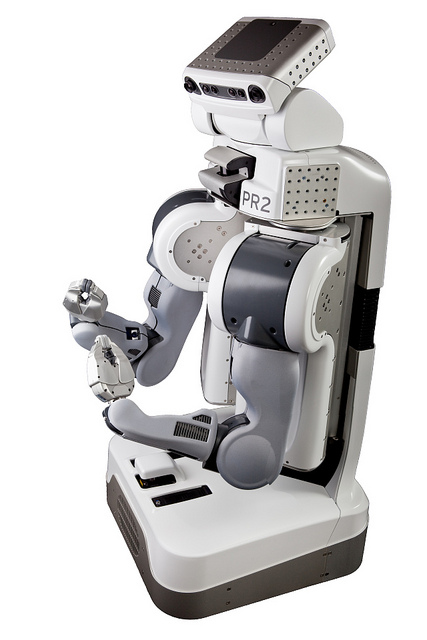
\includegraphics[width=3.5cm]{images/PR2-robot-2.jpeg}%
    };    
    \node[inner sep=0pt,scale=1.1] at (10.0,-2.5) {%
      Environnement
    };
  \end{tikzpicture}
}

\def\motivationgraph{
  \begin{tikzpicture}[remember picture, overlay]
    %
    \draw[color=darkred, left color=red, right color=red!60, 
      xshift=9cm,yshift=-2cm,
      drop shadow={ashadow, color=red!60!black}] 
    \arrow;
    \draw[color=darkblue, right color=blue, left color=blue!60,%
      xshift=9cm,yshift=-3cm, %
      drop shadow={ashadow, color=blue!60!black}]       
     [rotate=260] \arrow;
    %
    % Noeud sur le traitement du signal.
    \node [text centered, text width = 1.75cm, rectangle,draw,fill=blue!10!white] 
    (sensors)
    at (5.5,-0.25) {Traitement\\du signal};
    %
    % Repr�sentation de l'environnement
    \node [text centered, text width = 3.2cm, rectangle,draw,fill=blue!10!white] 
    (worldmap)
    at (2.0,-0.75) {Repr�sen    tation\\ de l'environnement};
    %
    % Contr�le
    \node [text centered, text width = 1.75cm, rectangle,draw,fill=blue!10!white] 
    (control) 
    at (5.5,-4.9) {Contr�le};    
    %
    % Planification de mouvement
    \node [text centered, text width = 2.5cm, rectangle,draw,fill=blue!10!white] 
    (motionplanning)
    at (2.25,-4.25) {Planification de mouvement};
    %
    % Planification de taches.
    \node [text centered, text width = 2.0cm, rectangle,draw,fill=blue!10!white] 
    (taskplanning)
    at (1,-2.5) {Planification de t�ches};          
    %
    % Physical relationship
    \draw[->,>=triangle 60,very thick,color=red] (hrp2) -- (sensors);
    \draw[->,>=triangle 60,very thick,color=red] (control) -- (hrp2);
  \end{tikzpicture}
}

\def\implementationgraph{
 
\begin{tikzpicture}[remember picture, overlay]
    \node [text centered, text width = 3cm] 
    at (4.5,0.5) {OpenCV - PCL};

    \node [text centered, text width = 3.2cm] 
    at (1.0,0.0) {OctoMap};

    \node [text centered, text width = 3.5cm] 
    at (4.75,-5.45) {KLD - iTask - SoT};

    \node [text centered, text width = 2.5cm] 
    at (1.25,-5.0) {MovIt};

    \node [text centered, text width = 2.0cm] 
    at (-0.75,-3.25) {SMACH};   
 \end{tikzpicture}
}       

\def\deploymentgraph{
 
\begin{tikzpicture}[remember picture, overlay]
    \node[text centered, text width = 3cm] 
    (pcvision) at (4.25,0.5) 
    {PC - Vision};

    \node[text centered, text width = 3.2cm] 
    (pcmapping) at (0.75,0.0) 
    {PC - Mapping};

    \node[text centered, text width = 3.5cm] 
    (pccontrol) at (4.3,-5.45) 
    {PC - Contr\^{o}le};

    \node[text centered, text width = 4.5cm] 
    (pcmotionplanning) at (1.05,-5.0) 
    {PC - Motion Planning};

    \node[text centered, text width = 4.5cm] 
    (pctaskplanning) at (-0.5,-3.25) 
    {PC - Task Planning};
 \end{tikzpicture}
}


\def\logicalrelationship{
 \begin{tikzpicture}[remember picture, overlay]        
   %
    % Logical relationship
      % Data flow
   \draw[<-,>=triangle 45,>=triangle 45] (control)--(sensors);
   \draw[->,>=triangle 45,>=triangle 45] (motionplanning)--(control); 
   \draw[->,>=triangle 45,>=triangle 45] (sensors)--(worldmap); 
   \draw[->,>=triangle 45,>=triangle 45] (worldmap) to[out=315,in=90] (motionplanning); 
   \draw[<-,>=triangle 45,>=triangle 45] (taskplanning) -- (worldmap);
   \draw[->,>=triangle 45,>=triangle 45] (taskplanning)--(motionplanning);
   \draw[->,>=triangle 45,>=triangle 45] (taskplanning) to[out=0,in=135] (control);
 \end{tikzpicture}
}

\def\softwarerelationship{
 \begin{tikzpicture}[remember picture, overlay]        
    %\draw[help lines] (-5,-5) grid (5,5);
    %\node at (0,0) {(0,0)};
    %
    % Software relationship
    % Bus logiciel.
    \node [text centered, text width = 2.0cm, rectangle,draw,fill=blue!20!white] 
    (softwarebus) at (3,-2.5) {Bus logiciel};          
    % 
    % Software bus
    \draw[<->,>=triangle 45,>=triangle 45] (control)--(softwarebus);
    \draw[<->,>=triangle 45,>=triangle 45] (motionplanning) -- (softwarebus); 
    \draw[<->,>=triangle 45,>=triangle 45] (worldmap)--(softwarebus); 
    \draw[<->,>=triangle 45,>=triangle 45] (taskplanning)--(softwarebus);
    \draw[<->,>=triangle 45,>=triangle 45] (sensors)--(softwarebus);
 \end{tikzpicture}
}
 
\def\rosecosystem{
  \begin{tikzpicture}[remember picture, overlay]        
     %\draw[help lines] (0,-3) grid (5,0);         
     %\node at (0,0) {(0,0)};
     \node at (-0.25,-0.5) {Support� :};
     \node at (2.0,-0.5) {\pgfuseimage{ros-ubuntu-logo}};
     \node at (0.25,-1.5) {Exp�rimentaux :};
  
     \node at ( 0.0,-2.5) {\pgfuseimage{ros-ubuntu-arm-logo}};
     \node at ( 2.0,-2.5) {\pgfuseimage{ros-os-x-homebrew-logo}};
     \node at ( 4.0,-2.5) {\pgfuseimage{ros-os-x-macports-logo}};
     
     \node at ( 0.0,-3.5) {\pgfuseimage{ros-yocto-logo}};
     \node at ( 2.0,-3.5) {\pgfuseimage{ros-debian-logo}};
     \node at ( 4.0,-3.5) {\pgfuseimage{ros-arch-linux-logo}};

     \node at ( 0.0,-4.5) {\pgfuseimage{ros-windows-logo}};
     \node at ( 2.0,-4.5) {\pgfuseimage{ros-angstrom-logo}};
     \node at ( 4.0,-4.5) {\pgfuseimage{ros-udoo-logo}};
     
  \end{tikzpicture}\\
}

\tikzstyle{roscode}=[text width=10cm,fill=blue!20,
                     thick,draw=blue!50]
\tikzstyle{roslist}=[text width=10cm]

\def\robotsecosystem{
  \begin{tikzpicture}[remember picture, overlay]        
     %\draw[help lines] (-6,-3) grid (5,0);         
     %\node at (0,0) {(0,0)};
     \node[right] at (-3.0,-0.3) {\tiny 01/05/2014 : 111 Robots support�s sur \url{http://wiki.ros.org/Robots}};
     \node[right] at (-3.0,-0.85)  {\tiny 01/05/2014 : 2048 Packages support�s sur \url{http://wiki.ros.org/Packages}};
  
     \node at (  0.0,-3.5) {\pgfuseimage{ros-nao}};
     \node at (  4.0,-3.5) {\pgfuseimage{ros-turtlebot}};
     \node at ( -4.0,-3.5) {\pgfuseimage{ros-motoman}};
     
  \end{tikzpicture}\\        
}
